\documentclass[14pt]{beamer}
\usepackage[utf8]{inputenc}
\usepackage[T1]{fontenc}
\usepackage{lmodern}
\usepackage{animate}
\usetheme{CambridgeUS} %default
\usepackage{graphicx}
\usepackage[absolute,overlay]{textpos}

\begin{document}
	\author[Will C. Forte]{Will C. Forte\\ (will.c.forte@rutgers.edu)}
	\title{Introduction to the\\ MuJoCo Simulator}
	%\subtitle{}
	%\logo{}
	\institute[Rutgers University]{Department of Mechanical Engineering\\Rutgers University–New Brunswick}
	\date[February 11, 2025]{February 11, 2025\\ N2E Robotics}
	%\subject{}
	%\setbeamercovered{transparent}
	%\setbeamertemplate{navigation symbols}{}
	\begin{frame}[plain]
		\maketitle
	\end{frame}
	
	\begin{frame}
		\frametitle{About Me}
		
		I am an undergraduate freshman in the Engineering Honors Academy and an aspiring roboticist. Currently, I work on legged robots and some simulations.
		\vspace{0.6cm}
		
		\begin{itemize}
			\item 2023 -- Intern at an NJIT robotics lab
			\item 2024 -- Graduated high school
			\item 2024 -- Intern at Prof. Burlion's UAV lab
			\item 2025 -- Intern at Prof. Yi's legged robot lab
		\end{itemize}

		\vspace{0.6cm}
		
		My personal project site is \texttt{willcforte.com}.
	\end{frame}
	
	\begin{frame}{My Research Interests}
		\begin{itemize}
			\item Bipedal and quadrupedal design/control
			\item UAV control
			\item Dynamical systems analysis
			\item Biomimetic design
		\end{itemize}
		\vspace{0.5cm}
		Ben Katz' MIT Mini Cheetah inspired me to do robotics.
		\begin{center}
			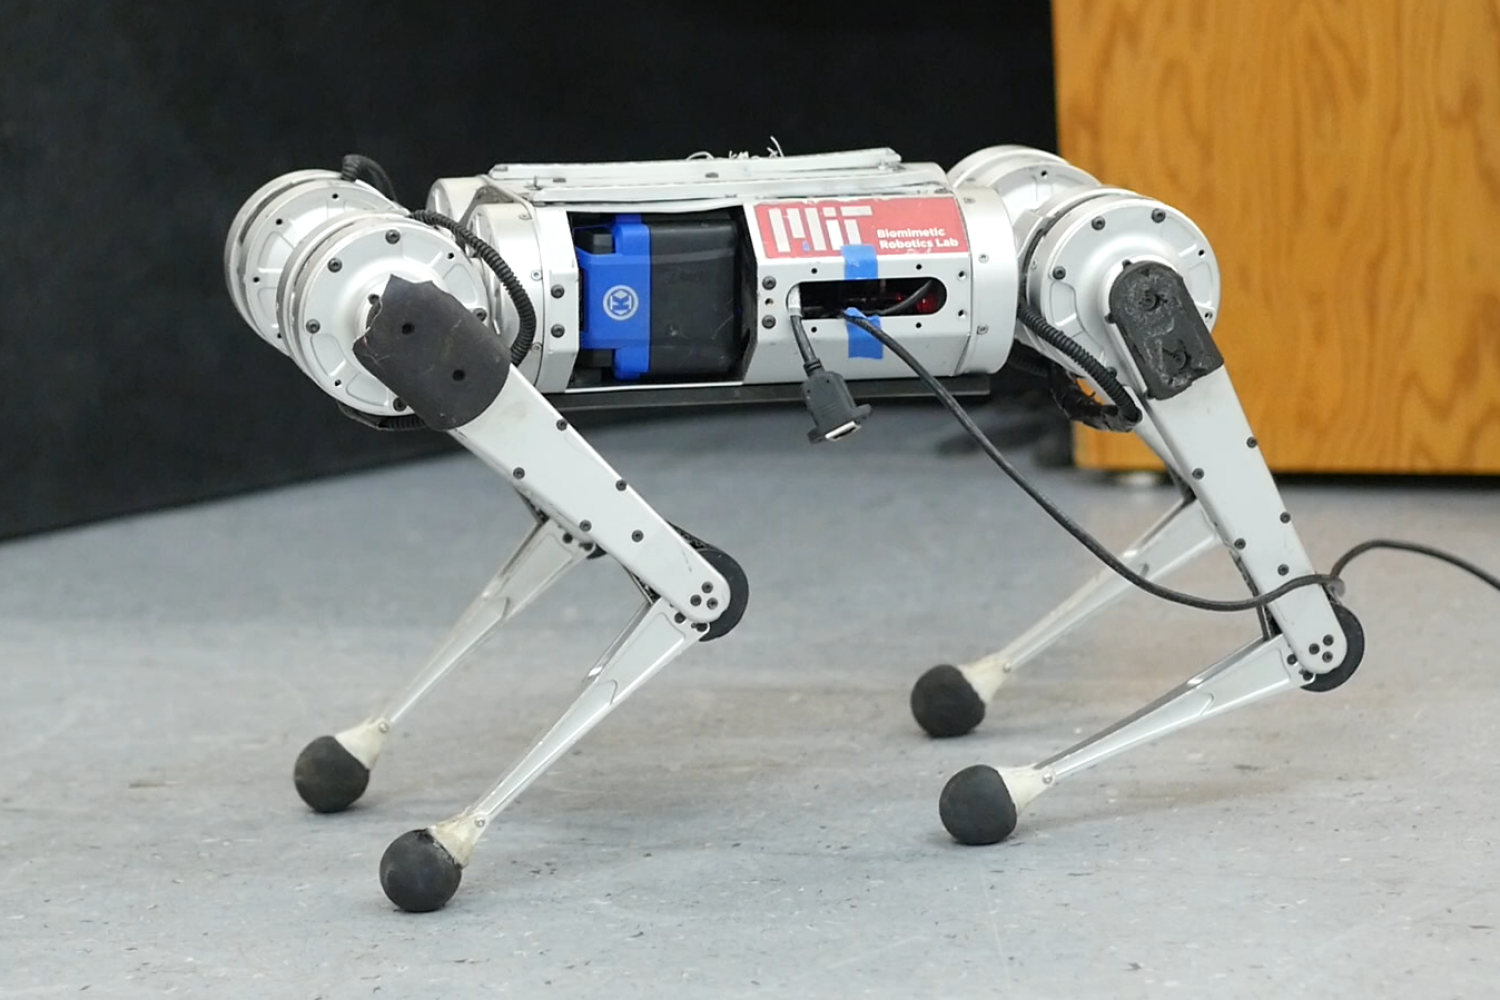
\includegraphics[height=15ex]{minicheetah-stand2.png}
			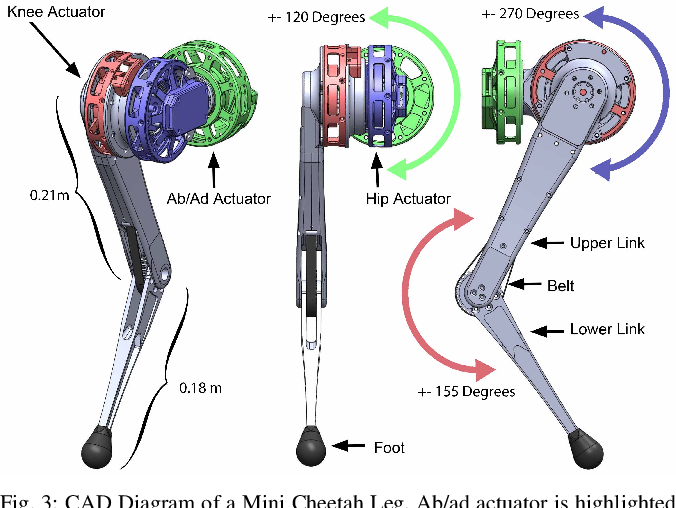
\includegraphics[height=15ex]{cheetah_leg.png}
		\end{center}
		\vspace{1cm}
	\end{frame}
	
	\begin{frame}
		\frametitle{DIY 12-Motor Quadruped \small{(Summer of 2023)}}
		
		\includegraphics[width=\linewidth]{quad_canon_prone.JPG}
	\end{frame}
	
	\begin{frame}
		\frametitle{My MuJoCo Simulation \small{w/ QR}}
		
		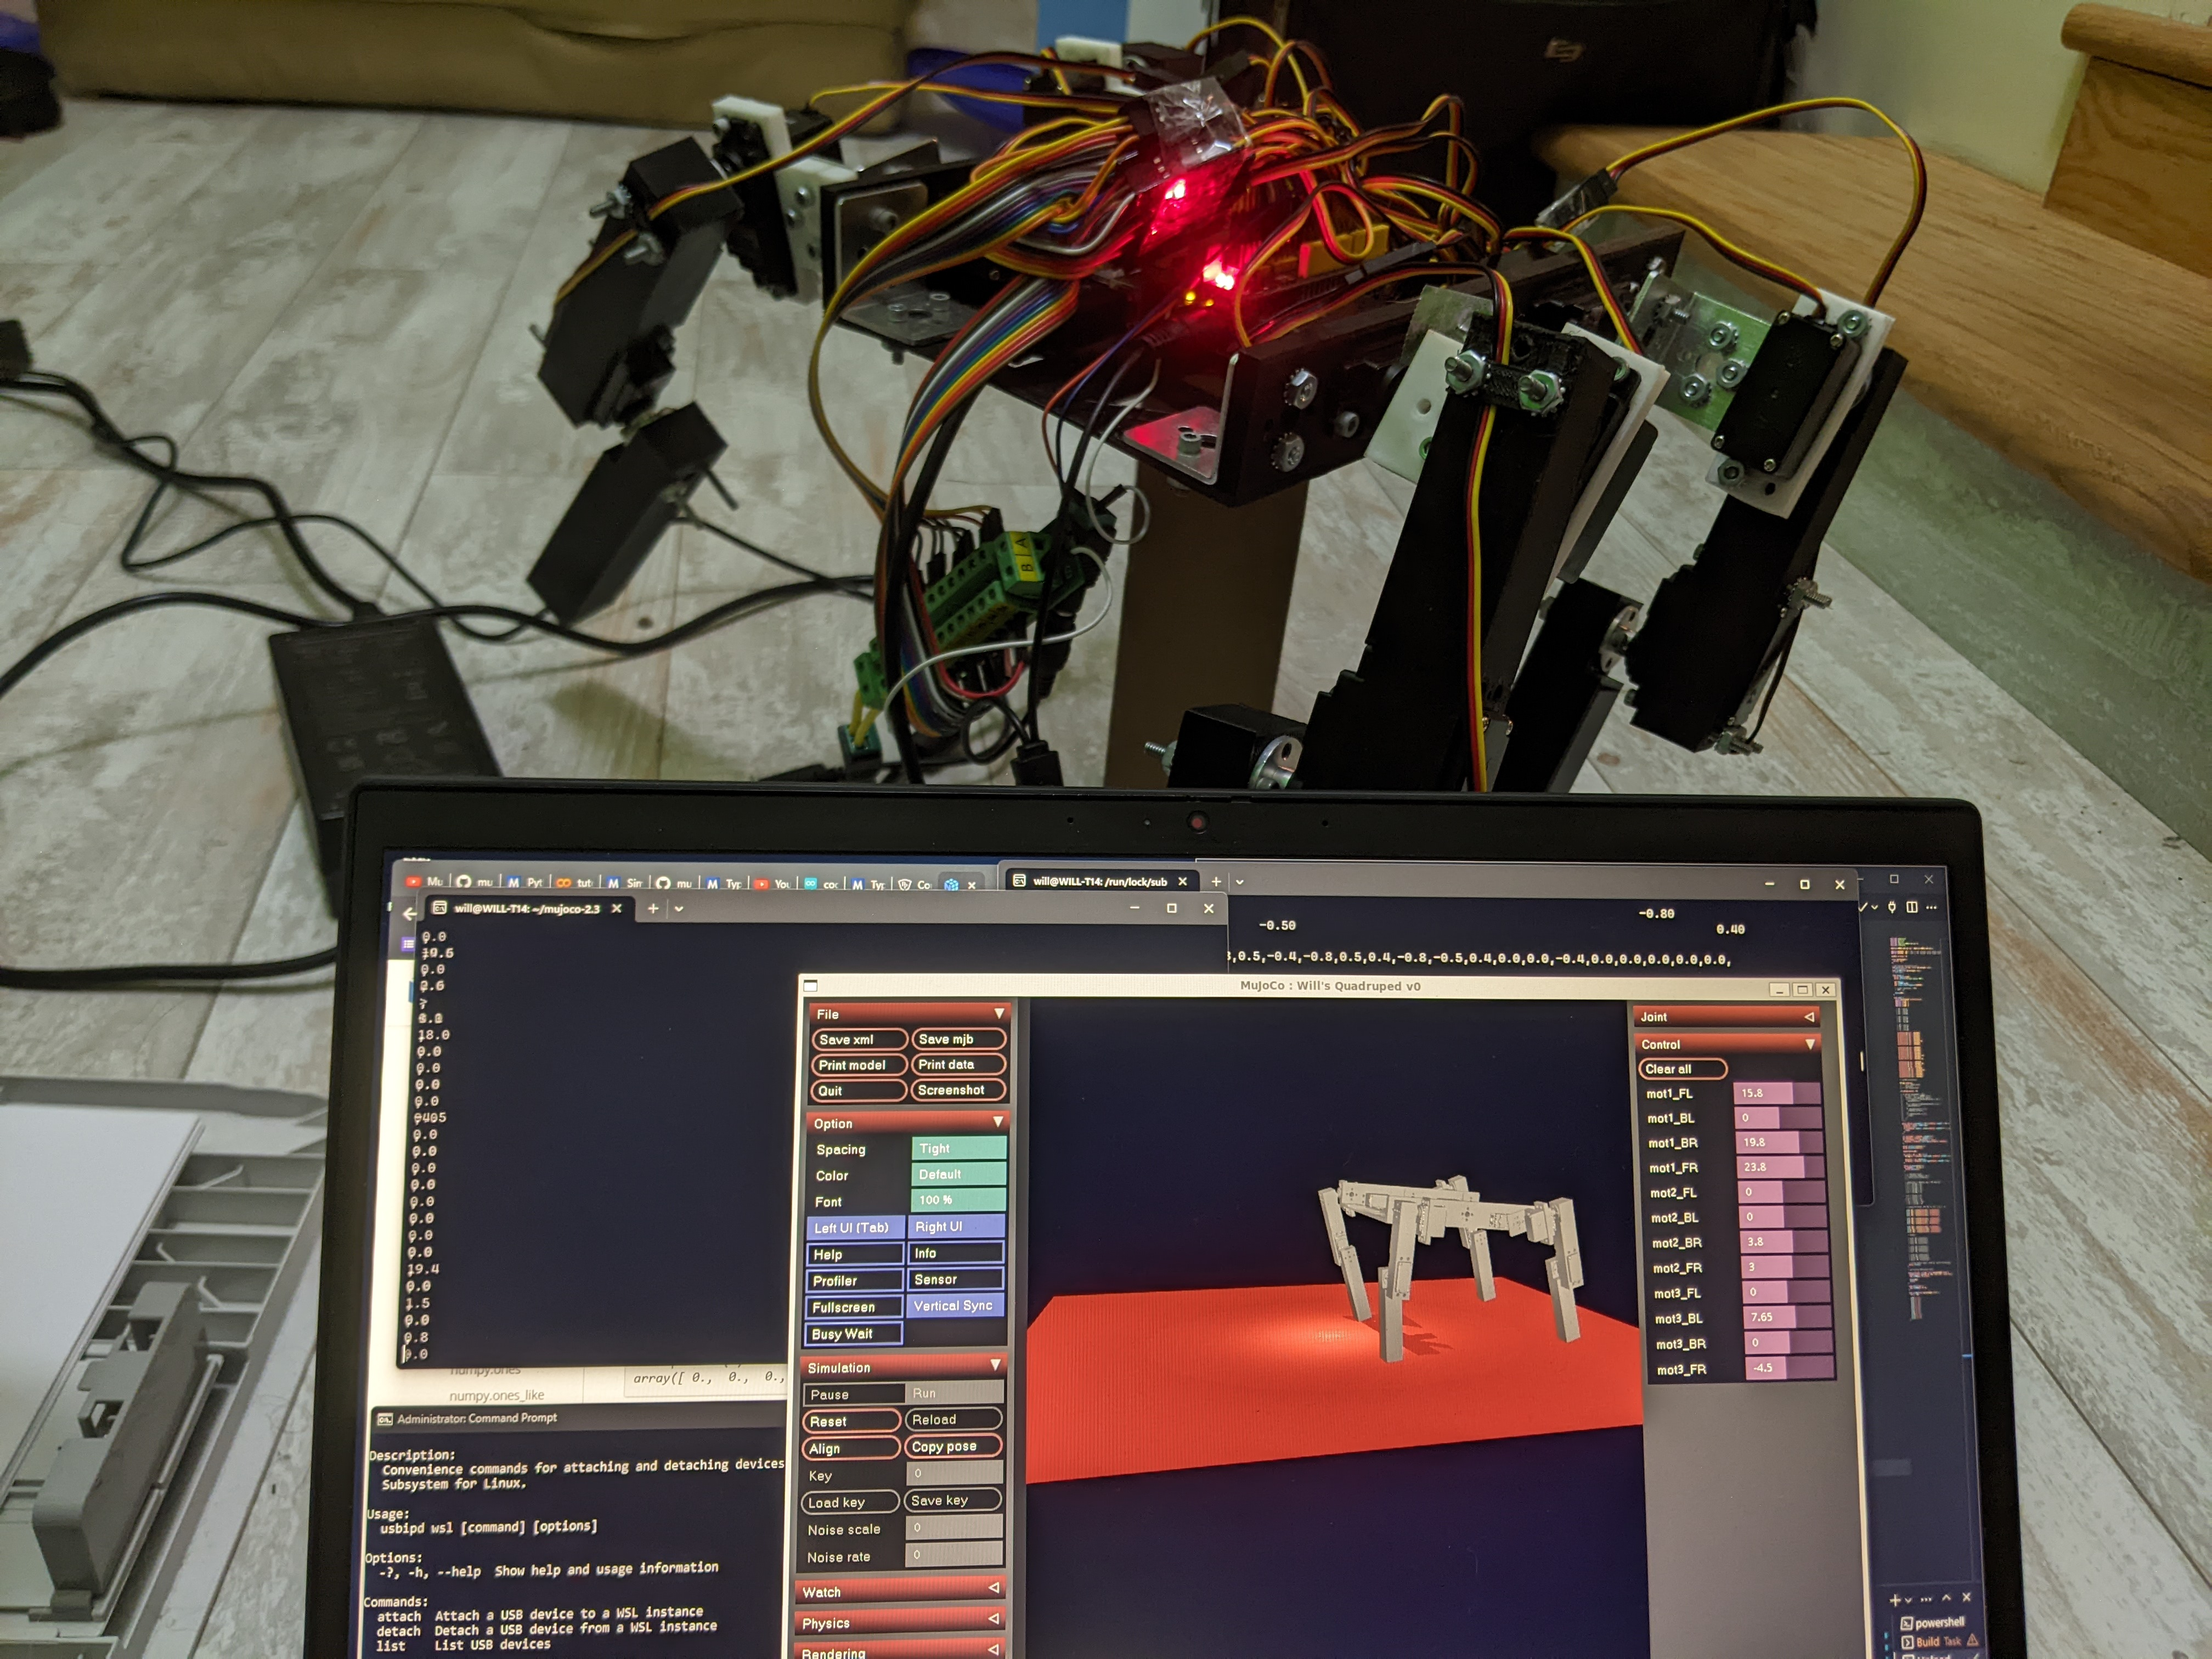
\includegraphics[width=\linewidth,trim={0 0 10cm 0},clip]{quadruped_v1_control.jpg}
		
		\begin{textblock*}{\textwidth}(0ex,7ex)
			
\includegraphics[width=4cm]{wcf_qr_cyberchef_mod8_m4_quartile.png} % Adjust width as needed
		\end{textblock*}
		
		
	\end{frame}
	
	\begin{frame}
		\frametitle{Why Simulate?}
		
		\begin{itemize}
			\item You don't have to buy a robot
			\item Break things with no consequences
			\item Easier than a real experiment
			\item Accurate sensors \& data collection
			\item It's fun!
		\end{itemize}
	\end{frame}
	
	\begin{frame}{What is MuJoCo?}
		MuJoCo is a robotics simulator developed by Emo Todorov of the University of Washington. It is maintained by Yuval Tassa's team at Google DeepMind.
		
		Its name is an acronym: $$\textbf{MuJoCo} \equiv \text{\textbf{Mu}lti \textbf{Jo}int (dynamics with) \textbf{Co}ntact}$$
		
		Of the current simulation options, I've found that MuJoCo is the easiest to use and demands the least computational power.
	\end{frame}
	
	\begin{frame}{Today's Objective}
		We are going to create a 2-joint manipulator that can be commanded to a certain position or follow a trajectory using MuJoCo and its Python library.
		% INSERT IMAGE OF FINAL SIMULATION
		\vspace{0.5cm}
		
		Let's get started! Feel free to ask any questions you may have as we go along.
	\end{frame}
	
	\begin{frame}{MuJoCo Simulation Example}
		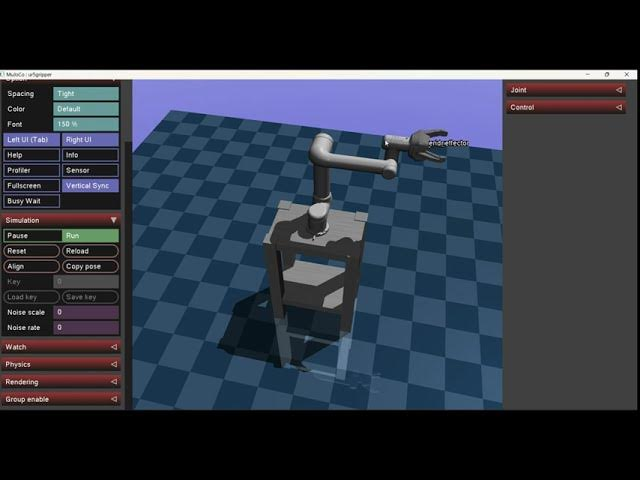
\includegraphics[width=\linewidth,trim={0 2cm 0 2cm},clip]{sizhe_tao_thumbnail.jpg}
		%image with parts of the GUI shown
		
		% what is mujoco not used for? Note that it does not work with ROS
	\end{frame}
	
	\begin{frame}{Downloading MuJoCo}
		MuJoCo can be installed from \texttt{mujoco.org}.
		% add nice image of mujoco website
		% DEMO - DOWNLOAD MUJOCO FOR UBUNTU
	\end{frame}
	
	\begin{frame}{Opening the Simulate Environment}
		Open \texttt{simulate.sh} to start the environment.
		
		\vspace{1cm}
		
		We need an XML file to describe our robot's structure.
	\end{frame}
	
	\begin{frame}{Workshop Repository}
		
\includegraphics[width=3.5cm,trim={0.5cm 0.5cm 0.5cm 0.5cm},clip]{workshop_qr.png}
		
		\vspace{0.2cm}
		
		https://github.com/willcforte/ Introduction-to-MuJoCo-Workshop/
		
		\vspace{0.2cm}
		
		Must be downloaded to your computer:
	
		\texttt{git clone https://github.com/willcforte/ Introduction-to-MuJoCo-Workshop/}
	\end{frame}
	
	\begin{frame}{Workshop Files}
		You can follow along using the instructions in the \texttt{exercises} folder.
		
		You can find the finished demo in the \texttt{reference} folder.
		
		A copy of this presentation is in the \texttt{docs folder}.
		
		% ADD THE PRESENTATION COPY
	\end{frame}
	
	\begin{frame}{Background: Degrees of Freedom (DoFs)}
		What is a degree of freedom (DoF)?
	\end{frame}
	
	\begin{frame}{Creating Our Simulated World in XML}
		Start with \texttt{./exercises/2R\_robotic\_arm.xml}
		
		To describe the hierarchical structure of a robot, MuJoCo uses XML, a format that uses angular brackets to nest elements within each other.
	\end{frame}
	
	\begin{frame}{Exercise 1: Joints and Bodies in MuJoCo}
		The \texttt{<worldbody>} contains everything in our world. Within it, we can place invisible \texttt{<body>} elements.
		
		\vspace{1cm}
		
		In MuJoCo, a body can contain any of three things:
		
		\vspace{1cm}
		
		1. A \texttt{<geometry>}, i.e. the meshes that you can see
		2. A \texttt{<joint>} which brings a degree of freedom to the body
		3. A child \texttt{<body>}, e.g. the next joint in the arm
	\end{frame}
	
	\begin{frame}{Background: PID Control}
		$$\text{PID Signal} \equiv P + I + D$$
		$$\equiv\text{Proportional}+\text{Integral}+\text{Derivative}$$
		$$ = k_p e(t) + k_i \int e(t)dt + k_d \frac{d}{dt}e(t)$$
	\end{frame}
	
	\begin{frame}{Exercise 2: Actuating Our Joints (Positional)}
		Positional servos are easy to use if you want to command a specific angle.
		
		Notice in the XML file that they even have a \texttt{kp} attribute. This is because the positional servo contains its own controller that keeps it at a certain angle.
	\end{frame}
	
	\begin{frame}{Demo: Controlling Actuators by GUI (Positional)}
		By uncommenting the \texttt{<position>} actuators, we can now control them in the GUI.
	\end{frame}
	
	\begin{frame}{Exercise 3: Actuating Our Joints (Motor)}
		Oftentimes in robotics, we use motors instead of positional servos.
		
		Motors apply accelerations, so we cannot control the particular angle.
	\end{frame}
	
	\begin{frame}{Demo: Controlling Actuators by GUI (Motor)}
		By uncommenting the \texttt{<motor>} actuators and commenting the \texttt{<position>} ones, we can control them in the GUI.
	\end{frame}
	
	\begin{frame}{Exercise 4: Using MuJoCo with Python}
		Make sure you have these dependencies: \texttt{wget}, \texttt{python3}, \texttt{git}.
	\end{frame}
	
	\begin{frame}{Exercise 5: Controlling a Positional Trajectory Using PID}
		We will be using \texttt{position\_PID.py}.
		
		\vspace{1cm}
		
		Try to experiment with different PID gains!
	\end{frame}
	
	\begin{frame}{Exercise 6: Controlling a Motor Trajectory Using PID}
		We will be using \texttt{motor\_PID.py}
		
		\vspace{1cm}
		
		Try to experiment with different PID gains!
	\end{frame}
	
	\begin{frame}{How can We Improve This Program?}
		Consider how humans command robots to go to a certain \emph{position}.
		
		\vspace{1cm}
		
		Robots, on the other hand, work best when given \emph{angles}.
	\end{frame}
	
	\begin{frame}{The Robot's Perspective}
		Current instruction method: we provide angles, which the robot uses to control itself.
		
		\vspace{1cm}
		
		State vector:
		
		$$\vec{x} = \begin{bmatrix}\theta_1 \\ \theta_2\end{bmatrix}$$
	\end{frame}
	
	\begin{frame}{The Human's Perspective}
		It would be more convenient for us to give a trajectory of positions.
		
		$$\vec{r}=\begin{bmatrix}r_x \\ r_y \end{bmatrix}$$
	\end{frame}
	
	\begin{frame}{Background: Inverse Kinematics}
		Going from positions to angles ($x \to\vec{r}$) is known as Inverse Kinematics.
	\end{frame}
\end{document}